%%%%%%%%%%%%%%%%%%%%%%%%%%%%%%%%%%%%%%%%%
% Journal Article
% LaTeX Template
% Version 1.4 (15/5/16)
%
% This template has been downloaded from:
% http://www.LaTeXTemplates.com
%
% Original author:
% Frits Wenneker (http://www.howtotex.com) with extensive modifications by
% Vel (vel@LaTeXTemplates.com)
%
% License:
% CC BY-NC-SA 3.0 (http://creativecommons.org/licenses/by-nc-sa/3.0/)
%
%%%%%%%%%%%%%%%%%%%%%%%%%%%%%%%%%%%%%%%%%

%----------------------------------------------------------------------------------------
%	PACKAGES AND OTHER DOCUMENT CONFIGURATIONS
%----------------------------------------------------------------------------------------

\documentclass[10pt]{article} % Single column

%\documentclass[twoside,twocolumn]{article} % Two column

\usepackage{blindtext} % Package to generate dummy text throughout this template 

\usepackage[sc]{mathpazo} % Use the Palatino font
\usepackage[T1]{fontenc} % Use 8-bit encoding that has 256 glyphs
\linespread{1.05} % Line spacing - Palatino needs more space between lines
\usepackage{microtype} % Slightly tweak font spacing for aesthetics

\usepackage[spanish]{babel} % Language hyphenation and typographical rules
\selectlanguage{spanish} 
\usepackage[hmarginratio=1:1,top=32mm,columnsep=20pt]{geometry} % Document margins
\usepackage[hang, small,labelfont=bf,up,textfont=it,up]{caption} % Custom captions under/above floats in tables or figures
\usepackage{booktabs} % Horizontal rules in tables

\usepackage{lettrine} % The lettrine is the first enlarged letter at the beginning of the text

\usepackage{enumitem} % Customized lists
\setlist[itemize]{noitemsep} % Make itemize lists more compact

\usepackage{abstract} % Allows abstract customization
\renewcommand{\abstractnamefont}{\normalfont\bfseries} % Set the "Abstract" text to bold
\renewcommand{\abstracttextfont}{\normalfont\small\itshape} % Set the abstract itself to small italic text

\usepackage{titlesec} % Allows customization of titles
\renewcommand\thesection{\Roman{section}} % Roman numerals for the sections
\renewcommand\thesubsection{\roman{subsection}} % roman numerals for subsections
\titleformat{\section}[block]{\large\scshape\centering}{\thesection.}{1em}{} % Change the look of the section titles
\titleformat{\subsection}[block]{\large}{\thesubsection.}{1em}{} % Change the look of the section titles

\usepackage{fancyhdr} % Headers and footers
\pagestyle{fancy} % All pages have headers and footers
\fancyhead{} % Blank out the default header
\fancyfoot{} % Blank out the default footer
\fancyhead[C]{Dise\~no y An\'alisis de Algoritmos. \textbf{Proyecto \# 1: La Pelota}} % Custom header text
\fancyfoot[RO,LE]{\thepage} % Custom footer text

\usepackage{titling} % Customizing the title section

\usepackage{hyperref} % For hyperlinks in the PDF

\usepackage{graphicx} % For images

\usepackage{pifont} % bullets

\usepackage{amsmath}

%\usepackage{algorithm}
%\usepackage{algorithmic}
%\usepackage{algorithm2e}

% Keywords command
\providecommand{\keywords}[1]
{
	\small	
	\vspace{0.5em}
	\noindent \textbf{\textit{Palabras clave --- }} #1
}


%----------------------------------------------------------------------------------------
%	TITLE SECTION
%----------------------------------------------------------------------------------------

\setlength{\droptitle}{-4\baselineskip} % Move the title up

\pretitle{\begin{center}\Huge\bfseries} % Article title formatting
	\posttitle{\end{center}} % Article title closing formatting
\title{\normalsize{Dise\~no y An\'alisis de Algoritmos }\\
	\Huge\bfseries Proyecto \# 1: La Pelota \\
} % Article title
\author{% 
	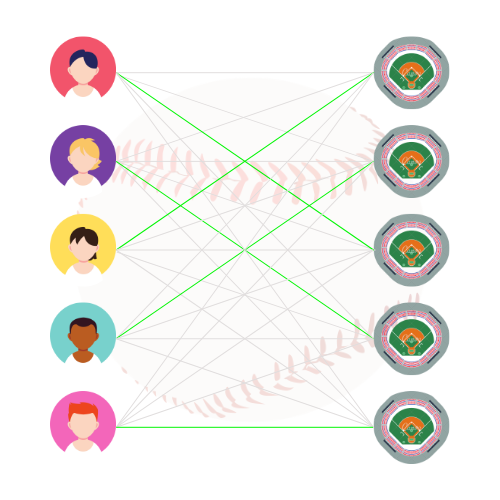
\includegraphics[width=15em]{logo.png}\\
	Laura Victoria Riera P\'erez\\
	Mari\'e del Valle Reyes \vspace{1em} \\
	\small Cuarto a\~no. Ciencias de la Computaci\'on. \\ % institution
	\small Facultad de Matem\'atica y Computaci\'on, Universidad de La Habana, Cuba \\ % institution
}
\date{\footnotesize \today } % Leave empty to omit a date


% Abstract configurations
\renewenvironment{abstract}
{\small
	\begin{center}
		\bfseries \abstractname\vspace{-.5em}\vspace{0pt}
	\end{center}
	\list{}{
		\setlength{\leftmargin}{1.5cm}%
		\setlength{\rightmargin}{\leftmargin}%
	}%
	\item\relax}
{\endlist}

\usepackage{amsthm}
\usepackage{amssymb}
\usepackage{todonotes} % \TODO
\usepackage{listings} % Code listings
\usepackage{xcolor}

\definecolor{backcolour}{rgb}{0.95,0.95,0.92}

\newcommand{\csl}[1]{\colorbox{backcolour}{\texttt{#1}}}

\newcommand{\imgcaption}[2]{\tiny \textbf{Figura #1.} #2.}

\newcommand{\mgc}[2][]{\colorbox{backcolour}{\texttt{\_\_#2\_\_#1}}}

\newcommand{\mgccapt}[1]{\texttt{\_\_#1\_\_}}

\newtheorem{thm}{Teorema}
\newtheorem{mydef}{Definici\'on}%[section]
\newtheorem{lem}{Lema}

\renewcommand{\qedsymbol}{\rule{0.7em}{0.7em}}



% Hyperlinks configurations
\hypersetup{
	colorlinks=true,
	linkcolor=black,
	filecolor=magenta,      
	urlcolor=cyan,
	pdftitle={Overleaf Example},
	pdfpagemode=FullScreen,
}

%----------------------------------------------------------------------------------------

\begin{document}
	% Print the title
	\maketitle
	
	%----------------------------------------------------------------------------------------
	%	ARTICLE CONTENTS
	%----------------------------------------------------------------------------------------
	
	\section{Repositorio del proyecto}
	
	\begin{center}
		\href{https://github.com/computer-science-crows/algorithms-design-and-analysis}{https://github.com/computer-science-crows/algorithms-design-and-analysis}
	\end{center}

	\section{Definici\'on inicial del problema} 
	
	Para un campeonato de pelota, el manager debe elegir de un conjunto de $ n $ personas, a su equipo de $ p $ jugadores, y a $ k $ espectadores especiales para que suban la moral del equipo.
	De cada persona $ i $, el manager conoce el valor que aporta a la moral del equipo $ a_i $ y el valor que aporta siendo situado en la posici\'on $ j $, $ s_{i,j} $. 
	Determine una alineación entre jugadores en el campo y espectadores de forma que el equipo tenga la mayor cantidad de valor acumulado posible.
	
	\section{Definici\'on en t\'erminos matem\'atico - computacionales}
	
	\subsection{Preliminares}
	
	\begin{mydef}
		Grafo bipartito
	\end{mydef}
	
	\begin{mydef}
		Grafo bipartito completo
	\end{mydef}
	
	\begin{mydef}
		Para un grafo no dirigido $G = (V,E)$, un emparejamiento es un subconjunto de aristas $M \in E$ tal que cada v\'ertice en $V$ tiene al menos una a arista incidente en $M$.
	\end{mydef}

	\begin{mydef}
		Otras definiciones
	\end{mydef}

	\begin{mydef}
		Camino M-alternativo
	\end{mydef}
	
	\begin{mydef}
		Camino M-aumentativo
	\end{mydef}
	
	\subsection{Problema de asignaci\'on}
	
	Dado un grafo bipartito completo ponderado $G = (V,E)$, donde $V = L \cup R$. Se asume que los v\'ertices de los conjuntos $L$ y $R$ contienen $n$ v\'ertice cada uno, por tanto el grafo contiene $n^2$ aristas. Para $l \in L$ y $r \in R$, se denota el peso de la arista $(l,r)$ como $w(l,r)$, lo cual representa ganancia de emparejar el v\'ertice $l$ con el v\'ertice $r$.
	
	El objetivo es encontrar el emparejamiento perfecto $M^*$ cuyas aristas tengan el peso m\'aximo total de todos los emparejamientos perfectos posibles. 
	
	Sea $w(M) = \sum_{(l,r) \in M} w(l,r)$ el peso total de las aristas en el emparejamiento $M$, se quiere encontrar el emparejamiento perfecto $M^*$ tal que,
	\[w(M*)=\text{max}\{w(M):M \text{ es un emparejamiento perfecto}\}\].
	
	A encontrar un emparejamiento perfecto de peso m\'aximo se le llama \textbf{problema de asignaci\'on}. Una soluci\'on del problema de asignaci\'on es un emparejamiento perfecto que maximice el costo total.
	
	En nuestro problema, el conjunto $V$ ser\'ia los nodos representando los jugadores y las posiciones, donde $L$ corresponder\'ia a los jugadores y $R$ a las posiciones. El conjunto $E$ lo conformar\'ian las aristas que van de cada nodo del conjunto $L$ a cada nodo del conjunto $R$. El peso de cada arista ser\'ia $s[i][j] + a[i]$.
	
	\section{Posibles soluciones investigadas}
	
	\section{L\'inea de pensamiento}
	\subsection{Backtrack}
	\subsection{Greedy}
	\subsection{Simplex}
	\subsection{Max flow min cut para mayor emparejamiento}
	No maximiza segun costos de aristas
	
	Se decidi\'o implementar el Hungarian por ser la solucion existente que resuelve lo pensado. 
	
	
	
	
 
	\section{Algoritmo H\'ungaro}
	
	El método Húngaro es un algoritmo de optimización-combinatoria que resuelve el problema de asignación en tiempo polinomial.
	
	En vez de trabajar con un grafo bipartito completo $G$, el algoritmo H\'ungaro trabaja con un subgrafo de $G$ llamado \textbf{subgrafo de igualdad}. El subgrafo de igualdad depende de asignar un atributo $h$ a cada v\'ertice. El atributo $h$ se llama \textbf{etiqueta} del v\'ertice. Se dice que $h$ es un \textbf{etiquetado de vértice factible} de $G$ si $l.h + r.h \geq w(l,r)$ para todo $l \in L$ y $r \in R$. Un etiquetado de v\'ertice factible siempre existe, como el \textbf{etiquetado de v\'ertice por defecto} dado por
	\begin{align}
		\label{eq:defecto}
		l.h &= \text{max} \{w(l,r):r \in R\} &\text{para todo } l \in R,\\
		r.h &= 0 &\text{para todo } r \in R 
	\end{align}

	Dado un etiquetado de v\'ertice factible $h$, el \textbf{subgrafo de igualdad} $G_h = (V, E_h)$ de $G$ consiste de los mismos v\'ertice de $G$ y el subconjunto de aristas $E_h = \{(l,r) \in E: l.h + r.h = w(l,r)\}$.
	
	El subgrafo de igualdad puede cambiar en el tiempo y tiene la propiedad que cualquier emparejamiento perfecto en el subgrafo de igualdad es tambi\'en una soluci\'on \'optima del problema de asignaci\'on como se demuestra en el siguiente teorema.
	\begin{thm} \cite{introduction}
		\label{thm: emparejamiento}
		Sea $G=(V,E)$, donde $V = L \cup R$, un grafo bipartito completo donde cada arista $(l,r) \in E$ tiene peso $w(l,r)$. Sea $h$ un etiquetado de v\'ertice factible de $G$ y $G_h$ el subgrafo de igualdad de $G$. Si $G_h$ contiene un emparejamiento perfecto $M^*$, entonce $M^*$ es una soluci\'on \'optima del problema de asignaci\'on $G$. 
		
	\end{thm}

	\begin{proof}
		Si $G_h$ tiene un emparejamiento perfecto $M^*$, entonces debido a que $G_h$ y $G$ tienen el mismo conjunto de v\'ertices, $M^*$ es tambi\'en un emparejamiento perfecto en $G$. Debido a que cada arista de $M^*$ pertenece a $G_h$ y cada v\'ertice tiene exactamente una arista incidente del emparejamiento perfecto, entonces se tiene
		
		\begin{align}
			w(M*) &= \sum_{(l,r) \in M*} w(l,r)\\
			&= \sum_{(l,r) \in M^*}(l.h + r.h) &\text{(porque todas las aristas de $M^*$ pertenecen a $G_h$)}\\
			&= \sum_{l \in L}l.h + \sum_{r \in R} r.h &\text{(porque $M^{*}$ es un emparejamiento perfecto)}\\
		\end{align} 
		
		Sea $M$ un emparejamiento perfecto cualquiera de $G$, se tiene
		
		\begin{align}
			w(M) &= \sum_{(l,r) \in M} w(l,r)\\
			&\leq \sum_{(l,r) \in M} (l.h + r.h) &\text{(porque $h$ es un etiquetado de v\'ertice factible)}\\
			&= \sum_{l \in L} l.h + \sum_{r \in R} r.h &\text{(porque $M$ es un emparejamiento perfecto)}
		\end{align}
		Entonces se tiene
		\begin{equation}
			w(M) \leq \sum_{l \in L} l.h + \sum_{r \in R} r.h = w(M^*),
		\end{equation}
		por tanto $M^*$ es un emparejamiento perfecto de m\'aximo costo en $G$.
	\end{proof}

	Entonces, el objetivo del algoritmo es encontrar un emparejamiento perfecto en un subgrafo de igualdad. 

\subsection{Explicaci\'on del algoritmo}

%El algoritmo H\'ungaro repetidamente modifica el emparejamiento y las etiquetas de v\'ertices en orden de alcanzar su objetivo.

El algoritmo H\'ungaro empieza con un etiquetado de v\'ertice factible $h$ que es el de defecto \ref{eq:defecto} y cualquier emparejamiento $M$ en el subgrafo de igualdad $G_h$.  En la resoluci\'on de este problema se utiliz\'o un algoritmo de emparejamiento maximal greedy. Luego, el algoritmo repetidamente encuentra un \textbf{camino $M$-aumentativo} $P$ en $G_h$ utilizando una variante de B\'usqueda Primero a lo Ancho (\textit{en ingl\'es}, \textbf{BFS}). 

 El algoritmo BFS empieza la b\'usqueda desde todos los v\'ertices no saturados de $L$, los cuales al inicio se insertan en la cola $Q$. La condici\'on de parada es que se descubra alg\'un v\'ertice no saturado de $R$, ya que un camino $M$-aumentativo es aquel que empieza en un v\'ertice no saturado de $L$ y termina en un v\'ertice no saturado de $R$, tomando aristas no saturadas de $L$ a $R$ y aristas saturadas de $R$ a $L$. El resultado del algoritmo es un bosque primero a lo ancho $F = (V_f, E_f)$, donde cada v\'ertice no saturado de $L$ es ra\'iz de alg\'un \'arbol de $F$.


Si la b\'usqueda de un camino $M$-aumentativo falla, se debe actualizar el etiquetado de v\'ertice factible para adicionar a $G_h$ al menos una arista nueva.

Una vez encontrado un camino $M$-aumentativo, actualiza el emparejamiento para que este sea la diferencia sim\'etrica de $M$ y $P$, incrementando as\'i el tama\~no del emparejamiento.  Mientras haya alg\'un subgrafo de igualdad que contenga un camino $M$- aumentativo, el tama\~no del emparejamiento puede incrementar, hasta que un emparejamiento perfecto se logre.

	Existen casos en los que la cola $Q$ se vac\'ia sin que se halla llegado a encontrar un v\'ertice no saturado de $R$ que conforme un camino $M$-aumentativo. Cuando esto ocurre, el algoritmo H\'ungaro actualiza el etiquetado de v\'ertices factible $h$ de acuerdo al siguiente lemma.
	
	\begin{lem}
		\cite{introduction}
		Sea $h$ un etiquetado de v\'ertice factible en el grafo bipartito completo G con el grafo de igualdad $G_h$, y se $M$ un emparejamiento para $G_h$ y $F$ el bosque constru\'ido a partir de una B\'usqueda Primero a lo Ancho (en ingl\'es, BFS) sobre el subgrafo de igualdad $G_h$. Entonces, la etiqueta $h'$,
		\begin{equation}
			v.h' =  \left\{
			\begin{array}{ll}
				v.h-\delta & \text{si $v \in F_l$}, \\
				v.h+\delta & \text{si $v \in F_r$}, \\
				v.h & e.o.c \\
			\end{array} 
			\right.
		\end{equation}				
		donde 
		\begin{equation}
			\label{eqn:delta}
		\delta = min\{l.h + r.l - w(l,r): l\in F_l, r \in F_r\}
		\end{equation}
		con $F_l = L \cap V_f$ y $F_r = R \cap V_f$ son v\'ertices del bosque $F$ que pertenecen a $L$ y a $R$, respectivamente, es una etiqueta de v\'ertice factible para $G$ con las siguientes propiedades:
		\begin{enumerate}
			\item Si (u,v) es una arista de bosque F para $G_h$, entonces (u,v) $\in E_{h'}$.
			\item Si (l,r) pertenece al emparejamiento M para $G_h$, entonces (l,r) $\in E_{h'}$.
			\item Existen v\'ertices $l \in F_l$ y $r \in R - F_r$ tales que (l,r) $\notin E_h$, pero (l,r) $\in E_{h'}$.  
		\end{enumerate} 
	\end{lem}
	\begin{proof}
		Primero se demuestra que $h'$ es un etiquetado de v\'ertice factible para $G$. Debido a que $h$ es un etiquetado de v\'ertice factible, se tiene $l.h + r.h \geq w(l,r)$ para todo $l \in L$ y $r \in R$. Para que $h'$ no sea un etiquetado de v\'ertice factible, entonces se necesitar\'ia que $l.h' + r.h' < l.h + r.h$ para alg\'un $l \in L$ y $r \in R$. La \'unica forma en que esto pudiera ocurrir ser\'ia para alg\'un $l \in F_l$ y $r \in R-F_r$. En esta instancia, la cantidad de decrecimiento es igual a $\delta$, entonces $l.h' + r.h' = l.h - \delta + r.h$. Por ecuaci\'on \ref{eqn:delta}, se tiene que $l.h - \delta + r.h \geq w(l,r)$ para cualquier $l \in F_l$ y $r \in R - F_r$, por tanto $l.h' + r.h' \geq w(l,r)$. Para cualquier otra arista, se tiene $l.h' + r.h' \geq l.h + r.h \geq w(l,r)$. Por tanto, $h'$ es un etiquetado de v\'ertice factible.
		
		Ahora se mostrar\'a la veracidad de las propiedades:
		
		\begin{enumerate}
			\item Si $l \in F_l$ y $r \in F_r$, entonces se tiene $l.h' + r.h' = l.h + r,h$ debido a que $\delta$ se adiciona a la etiqueta de $l$ y se substrae de la etiqueta de $r$. entonces, si una arista pertenece a $F$ para el grafo $G_h$, tambi\'en pertenece a $G_{h'}$.
			\item Se afirma que para el momentp en que el algoritmo H\'ungaro computa el nuevo etiquetado de v\'ertice factible $h'$, para toda arista $(l,r) \in M$, se tiene que $l \in F_l$ si y solo s\'i $r \in F_r$. 
			
			Para demostrar por qu\'e, se considera el v\'ertice saturado $r$ y la arista $(l,r) \in M$. 
			
			Primero se supone que $r \in F_r$, entonces la b\'usqueda encuentra $r$ y lo pone en la cola. Cuando $r$ se remueve de la cola, $l$ es descubierto, entonces $l \in F_l$. 
			
			Luego se supone que $r \notin F_r$, por tanto $r$ no se ha descubierto. Se demostrar\'a que $l \notin F_l$. La \'unica arista en $G_h$ que entra $l$ es $(r,l)$, y dado que $r$ no se ha descubierto, la b\'usqueda no ha tomado esta arista; si $l \in F_l$, no es por la arista ($r,l$). La \'unica otra forma que un v\'ertice en $L$ puede estar en $F_l$ es si es ra\'iz de la b\'usqueda, pero solo v\'ertices no saturados de $L$ son ra\'ices y $l$ est\'a saturado. Por tanto, $l \notin F_l$ y la afirmaci\'on se cumple.
			
			Se conoce que para $l \in F_l$ y $r \in F_r$ se cumple $l.h' + r.h' = l.h + r.h$. En caso contrario, cuando $l \in L-F_l$ y $r \in R-F_r$, se tiene que $l.h' = l.h$ y $r.h'=r.h$, entonces $l.h' + r.h' = l.h + r.h$. Por tanto, si la arista $(l,r)$ est\'a en el emparejamiento $M$ para el grafo $G_h$, entonces $(l,r) \in E_{h'}$.
			\item Sea $(l,r)$ una arista que no pertenece a $E_h$, tal que $l \in F_l$, $r \in R-F_r$ y $\delta = l.h + r.h - w(l,r)$. Entonces, por definici\'on de $\delta$, existe al menos una de esas arista. Luego, se tiene 
			
			\begin{align*}
				l.h' + r.h' &= l.h - \delta + r.h\\
				&= l.h - (l.h + r.h -w(l,r)) + r.h\\
				&= w(l,r)			
			\end{align*}
		y por tanto $(l,r) \in E_{h'}$. 
			
			
		\end{enumerate}
		
	\end{proof}

%	Es posible que una arista pertenezca a $E_h$ pero no a $E_{h'}$.\todo{demostrar esto ex 25.3-3}
	
	\subsection{Correctitud}
	
	\subsection{Complejidad Temporal}
	
	La complejidad temporal del algoritmo H\'ungaro implementado es $O(n^4)$, donde $|V|=2n$ y $|E|=n^2$ en el grafo original $G$.
	
	
	
	
	
	
	\subsection{Complejidad Espacial}
	
	\section{Generador de casos de prueba}
	
	\section{Tester}
	
	
	\section{Comparaci\'on de soluciones implementadas}
	
	\begin{thebibliography}
		a
		\bibitem{introduction} Cormen, Thomas H. y otros. \emph{Introduction to Algorithms}. 
		The MIT Press.
		4ta Edici\'on.		
		Cambridge, Massachusetts.
		2022.
	\end{thebibliography}
\end{document}


